\documentclass[12pt,a4paper]{article}

\usepackage{geometry}
\geometry{
  a4paper,
  total={170mm,257mm},
  left=20mm,
  right=20mm,
  top=20mm
}

\usepackage[utf8]{inputenc}
\usepackage[english, greek]{babel}
\usepackage[LGR, T1]{fontenc}

\usepackage{amsmath}
\usepackage{amsfonts}

\usepackage{graphicx}
\graphicspath{ {.} }

\usepackage{titlesec}
\titleformat{\section}{\large}{}{0em}{\textsc}[\titlerule]
\titleformat{\subsection}{\small}{}{0em}{\textbf}[]
\titleformat{\subsubsection}{}{}{0em}{\textit}[]

\title{Αλγόριθμοι και Πολυπλοκότητα}
\author{Γαβαλάς Νίκος, AM 03113121}
\date{Ιανουάριος 2019}

\begin{document}

  \maketitle

  \begin{center}
    \Large{4η Γραπτή Σειρά Ασκήσεων}
  \end{center}

  \section{Άσκηση 1}

    Ζητάμε όλα τα μονοπάτια \(p\) που ξεκινούν από το \(i\) και καταλήγουν σε
    κάποιο \(j\), με \(t(p) = \prod_{q=0}^{q=l-1}{t(q, q+1)} \ge β_l\).
    Το πρόβλημα μπορεί να λυθεί
    κατασκευάζοντας αρχικά έναν γράφο με κόμβους τους χρήστες και ακμές τις
    σχέσεις μεταξύ τους (δηλαδή αν ο χρήστης \(i\) έχει για τον χρήστη \(j\)
    τιμή εμπιστοσύνης \(t(i, j)\) τότε αναπαριστούμε τη σχέση αυτή με μία 
    κατευθυνόμενη ακμή \((i, j)\) και βάρος \(t(i, j)\)), και ύστερα αναζητώντας
    τα μονοπάτια από το \(i\) προς κάθε \(j\) με μήκος \(l \le k\)
    και συνολικό βάρος \( \ge β_l \) στον γράφο αυτόν.
    \\
    \\
    Για να μπορέσουμε να τρέξουμε {\latintext Bellman-Ford} και να βρούμε τα
    ζητούμενα μονοπάτια, κάνουμε πρώτα τα εξής: Πρώτον, αντί για το 
    \(p' = \arg\max_{p}{t(p)}\), αναζητούμε το \(p' = \arg\min_{p}{\{-\log
    {t(p)}}\}\) και αντί για βάρη ακμών \(t(i, j)\) χρησιμοποιούμε τις τιμές
    \( \log{\frac{1}{t(i, j)}} \).
    \\
    \\
    Με αυτές τις μετατροπές, μπορούμε να τρέξουμε τον {\latintext Bellman-Ford}
    που δίνει το συντομότερο μονοπάτι από τον \(i\) στον \(j\) με το πολύ \(m\)
    ακμές με την γνωστή αναδρομική σχέση:
    \[ D[j, m] = \min\{{D[j, m - 1],
      \min_{v : (v, j)\in E}\{ D[v, m - 1] + w(v, j) }\}\} \]
    \\
    Κάθε φορά που ανανεώνεται μια \(D[j, m]\) ελέγχουμε αν είναι \(\le 
    \log{\frac{1}{β_{m}}}\), και αν είναι, τότε ο \(j\) αποτελεί καλή πρόταση
    φίλου. Η πολυπλοκότητα είναι \(Ο(|V| + k|E|)\), αφού θέλουμε \(|V|\) χρόνο
    για να αρχικοποιήσουμε κάθε απόσταση \(D\) στο \(0\) και ύστερα \(k|Ε|\)
    χρόνο για να κάνουμε \(k\) επαναλήψεις που η καθεμία εξετάζει όλες τις
    ακμές. Αρκούν \(k\) γιατί τα μονοπάτια που αναζητούμε έχουν μέγιστο μήκος
    \(k\).

  \section{Άσκηση 2}

  \subsection{α)}

    Αν \(w(e) \in \{0, 1, ..., C\}\) με \(C\) σχετικά μικρό, μπορούμε να
    κάνουμε κάτι εμπνευσμένο από την {\latintext Counting Sort}. Κάνουμε
    {\latintext allocate} πίνακα \(Α\) μεγέθους \(nC\) (επειδή αυτή είναι η
    μέγιστη δυνατή απόσταση) με κάθε στοιχείο του πίνακα αυτού να είναι δείκτης
    σε λίστα κόμβων, και αρχικοποιούμε και έναν δείκτη \(i\) στην αρχή
    του πίνακα.
    \\
    \\
    Κάθε θέση του πίνακα αντιπροσωπεύει την απόσταση μεταξύ του κόμβου \(s\) 
    και καθενός εκ των στοιχείων της λίστας που δείχνει. Εκτελούμε κανονικά
    {\latintext Dijkstra}, με τη διαφορά ότι αντί να τοποθετούμε τους κόμβους
    σε λίστα προτεραιότητας, τους τοποθετούμε στην κατάλληλη λίστα από αυτές που
    δείχνουν τα στοιχεία του \(A\), βάσει απόστασης από τον \(s\),
    και σε κάθε βήμα προχωράμε τον \(i\) προς τα δεξιά, μέχρι το τέλος του
    πίνακα. Η τελική μορφή του \(Α\) περιέχει τις συντομότερες αποστάσεις
    από τον \(s\) προς οποιονδήποτε άλλον κόμβο.
    \\
    \\
    Ο αλγόριθμος αυτός έχει πολυπλοκότητα που υπολογίζεται ως εξής:
    Κάνουμε \(Ο(m)\) επισκεπτόμενοι κάθε ακμή από μία φορά κατά την εκτέλεση,
    και παράλληλα τον \(i\) τον μετακινούμε σε όλο το μέγεθος του \(Α\),
    άρα \(O(nC)\), οπότε σύνολο \(O(m + nC)\).
  
  \subsection{β)}

    O {\latintext Dijkstra} γνωρίζουμε ότι κάνει χρόνο
    \(Ο((n + m)\log{n})\), αν η ουρά προτεραιότητας είναι υλοποιημένη με
    {\latintext Binary Heap}, όπου ο όρος \(\log{n}\) προκύπτει από το χρόνο
    αναδιοργάνωσης του {\latintext Heap}. Αν έχουμε βάρη 
    \(w(e) \in \{0, 1, ..., 2^C\}\), τότε το βήμα αναδιοργάνωσης του σωρού δεν
    θα κάνει χρόνο \(n\), αλλά \(\log{2^C} = C\) γιατί δεν γίνεται να έχει
    ο σωρός ύψος μεγαλύτερο του \(\log{2^C}\) (αποδεικνύεται επαγωγικά).
    Επομένως έχουμε συνολικά
    εκτέλεση σε χρόνο \(Ο((n + m)C)\).

  \section{Άσκηση 3}

  \subsection{α)}

    Υποθέτουμε ότι \(c(e)\in \{0, 1\}\), και ζητάμε το μήκος του συντομότερου
    μονοπατιού με ακμές συνολικού κόστους το πολύ \(k\ge 1\). Το πρόβλημα
    αντιμετωπίζεται με τη κατασκευή ενός γράφου \(G'\) που προκύπτει από το
    αρχικό \(G\) ως εξής:
    \\
    \\
    Αρχικά φτιάχνουμε ένα γράφο \(G_0\) που έχει αντίγραφα
    όλων
    των κόμβων \(u\) του \(G\) ως \(u_0\) και αντίγραφα όλων των ακμών του \(G\)
    με κόστος \(0\). Μετά
    φτιάχνουμε έναν γράφο \(G_1\) που έχει επίσης αντίγραφα όλων των κόμβων του
    \(G\) αλλά οι ακμές του που έχουν κόστος \(1\), ξεκινάνε από αυτόν και
    καταλήγουν στους κόμβους
    του \(G_0\), και επίσης ο κόμβος εκκίνησης \(s_1\) ταυτίζεται με αυτόν του
    \(G_0\) (\(s_0 \equiv s_1\)).
    \\
    \\
    Με αυτόν τον τρόπο δημιουργούμε \(k\) επιπλέον του \(G_0\) γράφους, μέχρι
    τον \(G_k\), και τους ενώνουμε με ακμές κόστους \(1\) από τους κόμβους του
    \(G_i\) στους κόμβους του \(G_{i-1}, i = \{1, ..., k\}\). Σε αυτό το μεγάλο
    ενωμένο γράφημα λοιπόν, που αποτελεί το \(G'\), τρέχουμε {\latintext
    Dijkstra}, ο οποίος για κάθε κόμβο \(u_i, i=\{0, 1, ..., k\}\) θα υπολογίσει
    την ελάχιστου μήκους απόσταση με ακριβώς \(k\) κόστος. Επειδή ζητάμε
    την ελάχιστου μήκους απόσταση με το πολύ \(k\) κόστος, η τελική απάντηση
    δίνεται παίρνοντας το ελάχιστο εξ' αυτών για κάθε \(k\), δηλαδή το
    \(\min_{i \le k}u_i\).
    \\
    \\
    Η ορθότητα του αλγορίθμου αυτού βασίζεται στο ότι άπαξ και κατά την
    εκτέλεση από ένα γράφημα \(G_i\) οδηγηθούμε στο \(G_j\) με \(i > j\), δεν
    γίνεται να ((γυρίσουμε πίσω)) λόγω της τοποθέτησης των ακμών. Κάθε φορά
    δηλαδή που χρησιμοποιούμε ακμή κόστους \(1\), αλλάζουμε γράφο με αποτέλεσμα
    τελικά να εξασφαλίζεται ότι οι τελική απάντηση θα δοθεί με το πολύ \(k\)
    χρήσεις ακμών με κόστος \(1\). Οι ακμές κόστους \(0\) δεν επηρεάζουν σε
    κάτι.
    \\
    \\
    Η πολυπλοκότητα υπολογίζεται ως εξής: \(Ο(km)\) για την κατασκευή του \(G'\)
    και \(Ο(km + kn\log{(kn)})\) για την εκτέλεση του {\latintext Dijkstra}
    δίνουν συνολικό χρόνο \(Ο(km + kn\log{(kn)})\), η οποία είναι πολυωνυμική
    (της τάξης του \(O(mn + 2n^2\log{n})\)) αφού \(k < n\).

  \subsection{β)}

    To πρόβλημα θυμίζει το {\latintext 0-1 Knapsack}. Ακολουθώντας παρόμοια
    λογική με πριν, αφού το συνολικό κόστος θέλουμε να είναι \(\le C\),
    κατασκευάζουμε \(C + 1\) γράφους, τους \(G_i, i = \{0, 1, ..., C\}\), που
    έχουν κόμβους αντίγραφα \(u_i\) του αρχικού \(G\), και εννόνωνται με
    ακμές \(e_i = (u_i, v_{i + c(e)}), i \le C - c(e)\),
    για κάθε ακμή \(e = (u, v)\) του \(G\). Τέλος, ταυτίζουμε όλους τους κόμβους
    εκκίνησης μεταξύ τους.
    O γράφος που προκύπτει αποθηκεύει την πληροφορία του τρέχοντος κόστους
    στο επίπεδο \(i\).
    \\
    \\
    Αφού κατασκευάσουμε αυτόν τον γράφο, τρέχουμε σε αυτόν {\latintext Dijkstra}
    , και τέλος το συντομότερο μονοπάτι \(s-u\) με κόστος το πολύ \(C\) είναι το
    συντομότερο εκ των μονοπατιών \(s_0-u_i, \forall i \le C\).
    \\
    \\
    Σχετικά με την πολυπλοκότητα, θέλουμε \( Ο(Cn + Cm) \) για τη κατασκευή
    του γράφου και \(O(Cm + Cn\log{(Cn)})\) και για την εκτέλεση του 
    {\latintext Dijkstra}, άρα συνολικά \(O(Cm + Cn\log{(Cn)})\), όμως επειδή
    το \(C\) δεν φράσσεται από παράμετρο του προβλήματος, ο αλγόριθμος είναι
    όπως και το {\latintext 0-1 Knapsack} ψευδοπολυωνυμικού χρόνου.

  \section{Άσκηση 4}

    Στο πρόβλημα αυτό έχουμε \(m\) εταιρείες, η κάθε μία από τις οποίες
    (έστω η \(i\)-οστή) πληρώνει για \(c_i\) διαφημίσεις την ημέρα, που
    στοχεύουν σε ανθρώπους που ανήκουν σε κάποιες από \(k\) δημογραφικές
    κατηγορίες. Οι άνθρωποι αυτοί είναι στο σύνολό τους \(n\) και ο καθένας
    ανήκει σε το πολύ \(k\) δημογραφικές κατηγορίες.
    \\
    \\
    Θέλουμε να ξέρουμε αν υπάρχει τρόπος να προβάλλονται οι διαφημίσεις έτσι
    ώστε ο κάθε άνθρωπος να βλέπει μία διαφήμιση. Μπορούμε να λύσουμε το
    πρόβλημα με {\latintext Max Flow}. Αρχικά κατασκευάζουμε τον ακόλουθο
    γράφο:
    \begin{center}
      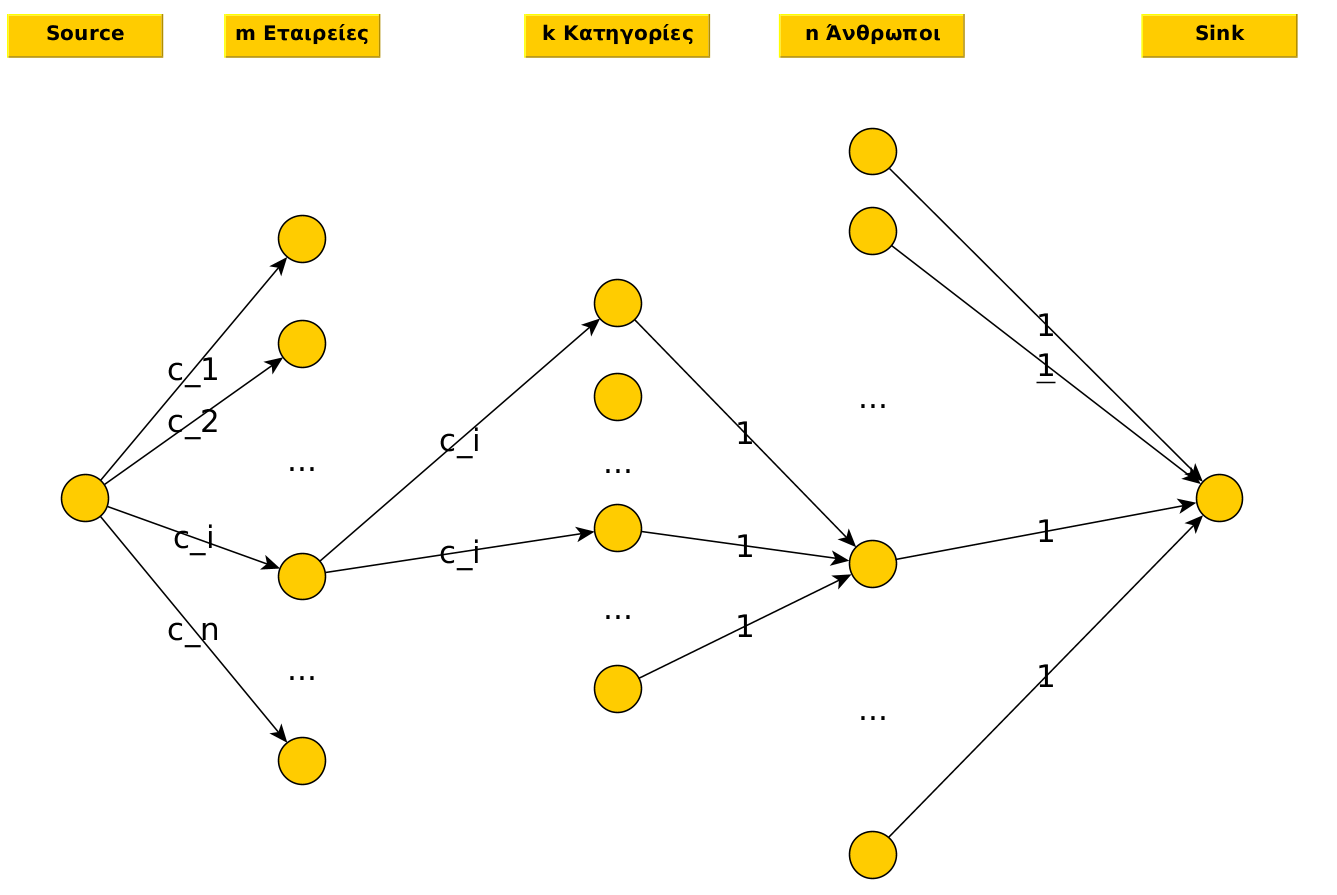
\includegraphics[width=\textwidth]{algo4a-graph.png}
    \end{center}
    , όπου πάνω στις ακμές είναι σημειωμένες οι χωρητικότητες. Βρίσκουμε ύστερα
    τη μέγιστη ροή με κάποιον αλγόριθμο {\latintext Max Flow}, και αν είναι ίση
    με \(n\), τότε μπορούμε να είμαστε σίγουροι ότι κάθε άνθρωπος είδε ακριβώς
    μία διαφήμιση. Για να βρούμε ποιοι ακριβώς βλέπουν για κάθε εταιρεία τις
    διαφημίσεις της, αρκεί να ακολουθήσουμε τις ροές από τον γράφο αφού τρέξουμε
    τον αλγόριθμο.
    \\
    \\
    Η πολυπλοκότητα αυτής της λύσης είναι αυτή του αλγορίθμου που θα
    χρησιμοποιήσουμε για το {\latintext Max Flow}, για παράδειγμα \(O(|E|n)\)
    αν χρησιμοποιήσουμε {\latintext Ford-Fulkerson}, συν όσο χρειάζεται για
    να κατασκευαστεί ο γράφος.

  \section{Άσκηση 5}

  \subsection{3-{\latintext Partition}}

    \underline{Είσοδος:} \(A=\{w_1, ..., w_n\}, w_i \in \mathbb{N}^{+}, w(A) 
    = \sum_{i \in
    A}{w_i} = 3k, k=\{0, 1, ...\}\)
    \\
    \underline{Ερώτηση:} \(\exists\) διαμέριση σε \(Α_1, Α_2, Α_3 : w(A_1)=
    w(A_2)=w(A_3)\)?
    \\
    \\
    Το πρόβλημα ανήκει στη κλάση {\latintext NP} γιατί αν μας δοθεί λύση
    μπορούμε να
    επιβεβαιώσουμε ότι είναι λύση σε γραμμικό χρόνο. Θα δείξουμε ότι είναι και
    {\latintext NP-hard} ως αναγωγή από το {\latintext Partition}.
    \\
    \\
    Έστω το σύνολο \(Α' = \{w_1, ..., w_n, \frac{\sum_{i=1}^{n}{w_i}}{2}\}\)
    \\
    Ευθύ: Από το {\latintext 3-Partition} παίρνουμε τρία υποσύνολα από το \(A'\)
    , ένα εκ των οποίων έχει μόνο το
    στοιχείο \(\frac{\sum_{i=1}^{n}{w_i}}{2}\) και
    άλλα δύο που αποτελούνται από στοιχεία του \(Α\) και δίνουν το
    {\latintext 2-Partition} αυτού.
    \\
    Αντίστροφο: Αν υπάρχει {\latintext 2-Partition}, προφανώς είναι και
    {\latintext 3-Partition}.

  \subsection{Άθροισμα Υποσυνόλου κατά Προσέγγιση}%- {\latintext Approximation
  %Subset Sum}}

    \underline{Είσοδος:} \(A=\{w_1, ..., w_n\}, w_i \in \mathbb{N}\) και
    \(x, B \in \mathbb{N}\) με \(B > x \ge 1\)
    \\
    \underline{Ερώτηση:} \(\exists S \subseteq A : B - x \le w(S) \le B\)?
    \\
    \\
    Το πρόβλημα ανήκει στη κλάση {\latintext NP} γιατί αν μας δοθεί λύση
    μπορούμε να
    επιβεβαιώσουμε ότι είναι λύση σε γραμμικό χρόνο. Θα δείξουμε ότι είναι και
    {\latintext NP-hard} ως αναγωγή από το {\latintext Subset Sum}.
    \\
    \\
    %Ευθύ:
    Έστω το \(A'=\{2w_1, 2w_2, ..., 2w_n\}\). Θέτουμε \(Β = 2W\) και
    \(x = 1\), οπότε γνωρίζουμε αν υπάρχει \(S \subseteq A: 2W -1 \le w(S) \le 
    2W\), δηλαδή αν υπάρχει \(S: w(S) = 2W -1\) ή \(w(S) = 2W\), όμως \(2W-1\)
    δεν γίνεται να υπάρχει γιατί το \(w(S)\) θα είναι άρτιος, οπότε γνωρίζουμε
    για ισότητα με \(2W\). Αυτό συνεπάγεται ότι γνωρίζουμε και τη λύση του
    {\latintext Subset Sum}, για τον πίνακα \(Α\) και παράμετρο \(W\).
    %\\
    %Αντίστροφο: Τρέχουμε το {\latintext Subset Sum} \(x+1\) φορές για παράμετρο
    %\(W \in [Β-x, x]\) και αποφαινόμαστε.

  \subsection{Κύκλος {\latintext Hamilton} κατά Προσέγγιση}% - {\latintext
  %Approximation Hamilton Cycle}}

    \underline{Είσοδος:} \(G(V, E)\) μη κατευθυνόμενο.
    \\
    \underline{Ερώτηση:} \(\exists\) κυκλική διαδρομή που διέρχεται από κάθε 
    κορυφή τουλάχιστον μία και το πολύ δύο φορές?
    \\
    \\
    Το πρόβλημα ανήκει στη κλάση {\latintext NP} γιατί αν μας δοθεί λύση
    μπορούμε να
    επιβεβαιώσουμε ότι είναι λύση σε γραμμικό χρόνο (ότι δηλαδή είναι κύκλος
    και περιλαμβάνει κάθε κορυφή από 1 ή 2 φορές). Θα δείξουμε ότι είναι και
    {\latintext NP-hard} ως αναγωγή από το {\latintext Hamilton Cycle}.
    \\
    \\
    Eυθύ: Κατασκευάζουμε τον γράφο \(G'\) με ίδιους κόμβους \(u\) με το \(G\)
    και ίδιες ακμές, και ύστερα του προσθέτουμε σε κάθε κόμβο \(u\) έναν
    κόμβο \(u'\) που συνδέεται με μία μοναδική ακμή. Τρέχοντας το
    {\latintext Approximation Hamilton Cycle}, ((υποχρεωνόμαστε)) να περάσουμε
    δύο φορές από κάθε κόμβο αφού για να συμπεριληφθεί στον τελικό κύκλο κάθε
    κόμβος \(u'\) πρέπει να περάσουμε δύο φορές από τον αντίστοιχο \(u\) \( (u 
    \rightarrow u' \rightarrow u)\). Τέλος παίρνουμε τη λύση για το
    {\latintext Hamiltonian Path} κόβοντας τους έξτρα κόμβους \(u'\).
    \\
    Αντίστροφο: Αν υπάρχει κύκλος {\latintext Hamilton}, υπάρχει και κύκλος
    κατά προσέγγιση.

  \subsection{Ικανοποιησιμότητα με Περιορισμούς}%- {\latintext Constrained SAT}}

    \underline{Είσοδος:} \(\phi = \bigwedge^{m}_{j=1}(\ell_{j1} \vee \ell_{j2}
    \vee \ell_{j3} \vee \ell_{j4}) \) λογική πρόταση σε {\latintext 4-CNF}
    \\
    \underline{Ερώτηση:} \(\exists\) ανάθεση λογικών τιμών ώστε κάθε όρος
    \(\ell_{j1} \vee \ell_{j2} \vee \ell_{j3} \vee \ell_{j4}\) να περιλαμβάνει
    τουλάχιστον ένα αληθές και ένα ψευδές {\latintext literal}?
    \\
    \\
    Το πρόβλημα ανήκει στη κλάση {\latintext NP} γιατί αν μας δοθεί λύση
    μπορούμε να
    επιβεβαιώσουμε ότι είναι λύση σε γραμμικό χρόνο. Θα δείξουμε ότι είναι και
    {\latintext NP-hard} ως αναγωγή από το {\latintext 3-SAT}.
    \\
    \\
    Έστω η λογική πρόταση \(\psi=\bigwedge^{m}_{j=1}(\ell_{j1} \vee \ell_{j2} 
    \vee \ell_{j3})\) και η \(\psi' = \bigwedge^{m}_{j=1}(\ell_{j1} \vee 
    \ell_{j2} \vee \ell_{j3} \vee x)\), όπου \(x\) λογική μεταβλητή που δεν
    εμφανίζεται αλλού.
    \\
    Ευθύ: Αν η \(\psi'\) ικανοποιείται για κάποια ανάθεση \(A\), τότε η ίδια
    ανάθεση ικανοποιεί και την \(\psi\), για \(x =false\), διαφορετικά αν
    \(x=true\), τότε την ικανοποιεί η ανάθεση που σχηματίζεται από τις λογικές
    αρνήσεις της \(Α\), άρα λύνεται το {\latintext 3-SAT}.
    \\
    Αντίστροφο: Αν υπάρχει ανάθεση που να ικανοποιεί την \(\psi\), τότε σημαίνει
    ότι τουλάχιστον ένας όρος από κάθε {\latintext clause} είναι \(true\),
    οπότε θέτοντας \(x=false\), ικανοποιείται και ο περιορισμός για
    την \(\psi'\).

  \subsection{Επιλογή Ανεξάρτητων Υποσυνόλων}% {\latintext 
  %(Set Packing)}}

    \underline{Είσοδος:} \(S=\{S_1, ..., S_m\}, S_i \subset U, U\) σύνολο με 
    \(n\) στοιχεία, \(k \in \mathbb{N}, 2 \le k \le m\)
    \\
    \underline{Ερώτηση:} Υπάρχουν \(k\) υποσύνολα από την \(S\) που να είναι ανά
    δύο ξένα μεταξύ τους?
    \\
    \\
    Το πρόβλημα ανήκει στη κλάση {\latintext NP} γιατί αν μας δοθεί λύση
    μπορούμε να
    επιβεβαιώσουμε ότι είναι λύση σε πολυωνυμικό χρόνο. Θα δείξουμε ότι είναι
    και {\latintext NP-hard} ως αναγωγή από το {\latintext MIS (Max
    Independent Set)}.
    \\
    \\
    Έστω γράφος \(G\) με \(m\) κορυφές, κατ' αντιστοιχία με τα σύνολα \(S_m\).
    Αν ένα από τα \(S_i\) τέμνεται με ένα \(S_j\), εισάγουμε ακμή \((i, j)\)
    στο \(G\).
    \\
    Ευθύ: Αν υπάρχουν \(k\) υποσύνολα του \(S\) που να είναι ανά
    δύο ξένα μεταξύ τους, τότε στον \(G\) υπάρχουν \(k\) κορυφές που δεν έχουν
    κοινές ακμές μεταξύ τους, άρα αποτελούν {\latintext Independent Set} με
    παράμετρο \(k\).
    \\
    Αντίστροφο: Αν ο \(G\) έχει \(k\) {\latintext Independent Sets}, δηλαδή
    \(k\) κόμβους που δεν έχουν κοινές ακμές μεταξύ τους, τότε τα
    αντίστοιχα \(S_i\) δεν τέμνονται, και άρα υπάρχουν \(k\) ανεξάρτητα εξ'
    αυτών.

  \subsection{Συντομότερο Μονοπάτι με Περιορισμούς}% {\latintext 
  %(Constraint Shortest Path)}}

    \underline{Είσοδος:} Κατευθυνόμενο \(G(V, E, w, c)\), \(s, t\) δύο κορυφές,
    \( w(e), c(e)\) μη-αρνητικοί ακέραιοι και \(W, C\) δύο επίσης μη-αρνητικοί
    ακέραιοι.
    \\
    \underline{Ερώτηση:} Υπάρχει \(s-t\) μονοπάτι στο \(G\) με συνολικό μήκος 
    \(\le W\) και συνολικό κόστος \(\le C\)?
    \\
    \\
    Το πρόβλημα ανήκει στη κλάση {\latintext NP} γιατί αν μας δοθεί λύση
    μπορούμε να
    επιβεβαιώσουμε ότι είναι λύση σε γραμμικό χρόνο. Θα δείξουμε ότι είναι
    και {\latintext NP-hard} ως αναγωγή από το {\latintext Knapsack}.
    \\
    \\
    Έστω \(n\) αντικείμενα με \(\beta_i, p_i\) το καθένα, και θέλουμε \(
    \sum{p_i} \ge P\), με τον περιορισμό \(\sum{\beta_i} \le B\), και έστω
    γράφος \(G\) με \(n\) κορυφές, τις \(u_i\).
    Προσθέτουμε στο \(G\) ακμές ως εξής:
    για κάθε κορυφή \(i\) προσθέτουμε δύο ακμές προς την \(i + 1\), η μία με 
    κόστος \(c_i=\sum_{i=0}^{n}{(p_i)} - p_i\) και μήκος \(w_i=\beta_i\) και η
    άλλη με κόστος \(\sum_{i=0}^{n}{(p_i)}\) και μήκος 0.
    Είναι εμφανές ότι η λύση του ενός προβλήματος για \(s=u_0, 
    t=u_n, W=B, C=n\sum_{i=0}^{n}{(p_i)} - P\)
    συνεπάγεται τη λύση του άλλου και αντίστροφα.

\end{document}
